\chapter{¿De qué están hechas las cosas?}\label{ch:g1:materials-around-us}

Mira una mesa de desayuno. Hay una cuchara, un vaso de leche, un
tenedor, una servilleta, un cuenco y un jersey colgado del respaldo de
una silla. Son muchas cosas, y cada una está hecha de algo: la cuchara
de madera, el tenedor de metal, el vaso de vidrio, la servilleta de
papel, el cuenco de plástico y el jersey de lana. Una mesa llena de
cosas, hechas con solo unos pocos \omterm{def:g1:materials-around-us:material}{materiales} distintos. De esos
\omterm{def:g1:materials-around-us:material}{materiales} trata este capítulo.

\begin{omfigure}
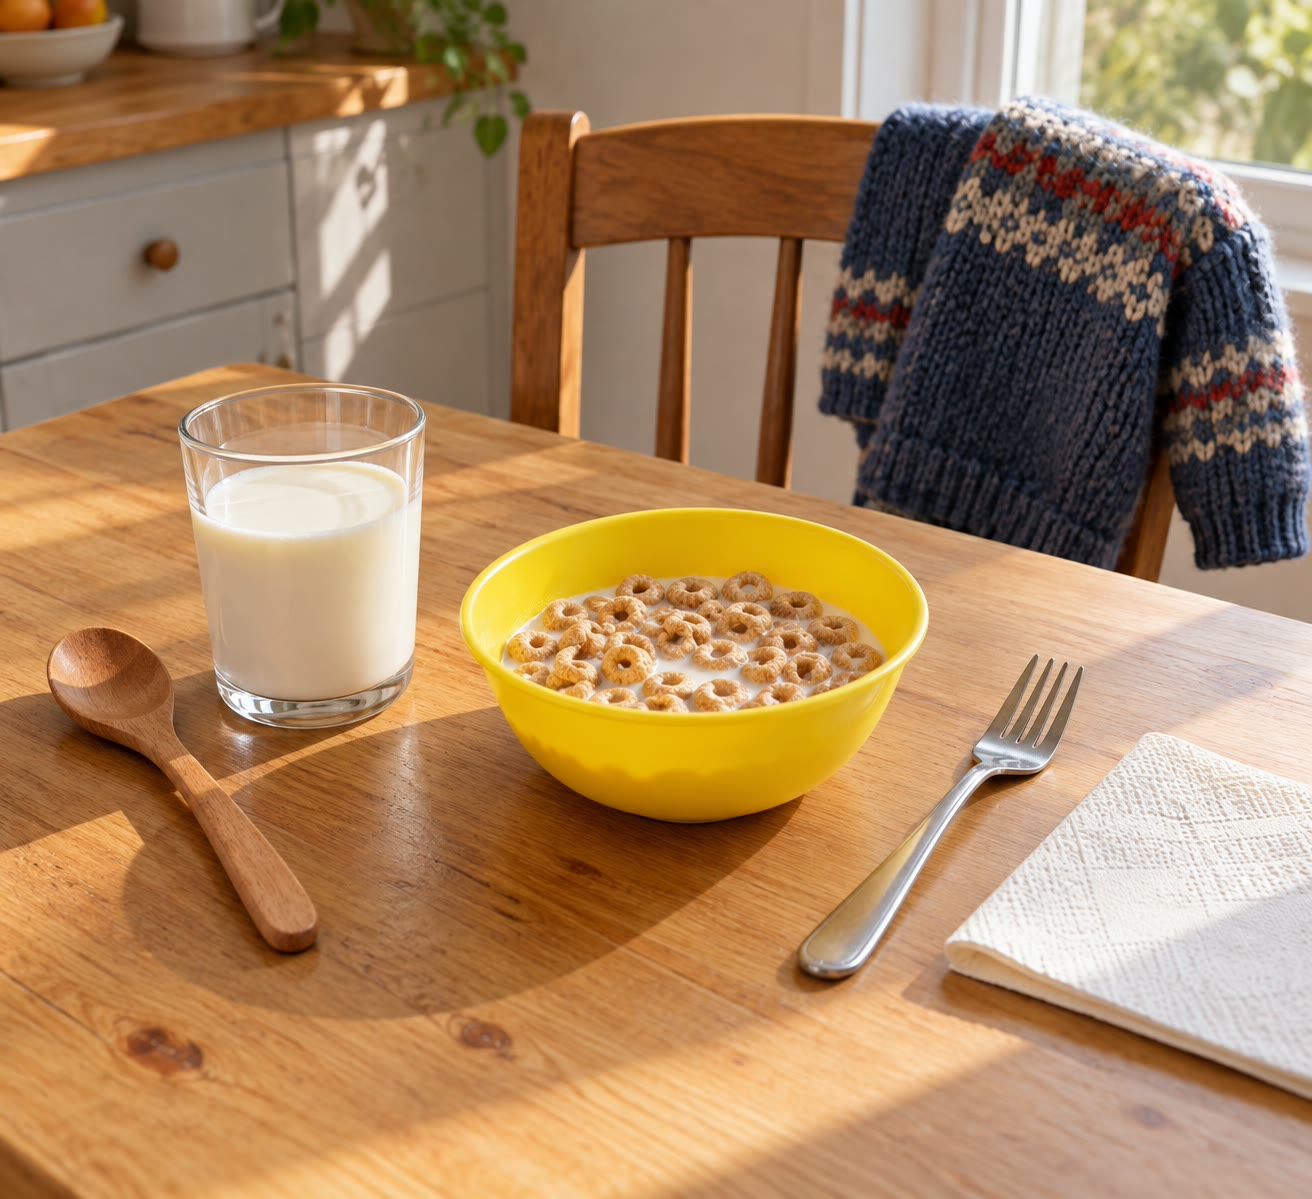
\includegraphics[width=0.62\linewidth]{images/book1/ai/g1-breakfast-table.jpg}

{\small Una mesa de desayuno: muchos \omterm{def:g1:materials-around-us:object}{objetos}, hechos de unos pocos \omterm{def:g1:materials-around-us:material}{materiales}.}
\end{omfigure}

\section{Objetos y materiales}

\begin{definition}[Objeto]\label{def:g1:materials-around-us:object}
Un \emph{objeto}\index{objeto} es una cosa que podemos ver y tocar, y
que a menudo podemos coger y usar: una cuchara, una silla, una pelota,
una ventana, un zapato.
\end{definition}

\begin{definition}[Material]\label{def:g1:materials-around-us:material}
El \emph{material}\index{material} de un \omterm{def:g1:materials-around-us:object}{objeto} es aquello de lo que
está hecho el \omterm{def:g1:materials-around-us:object}{objeto}. Una cuchara puede ser de madera, de metal o de
plástico: la cuchara es el \omterm{def:g1:materials-around-us:object}{objeto}, y la madera es el material.
\end{definition}

\begin{example}[Un objeto, tres materiales]\label{ex:g1:materials-around-us:spoons}
Hay tres cucharas una al lado de la otra. Tienen la misma forma y
sirven para lo mismo, así que son la misma clase de \omterm{def:g1:materials-around-us:object}{objeto}. Pero una es
de madera, otra de metal y otra de plástico: tres \omterm{def:g1:materials-around-us:material}{materiales} distintos.
\end{example}

\begin{omfigure}
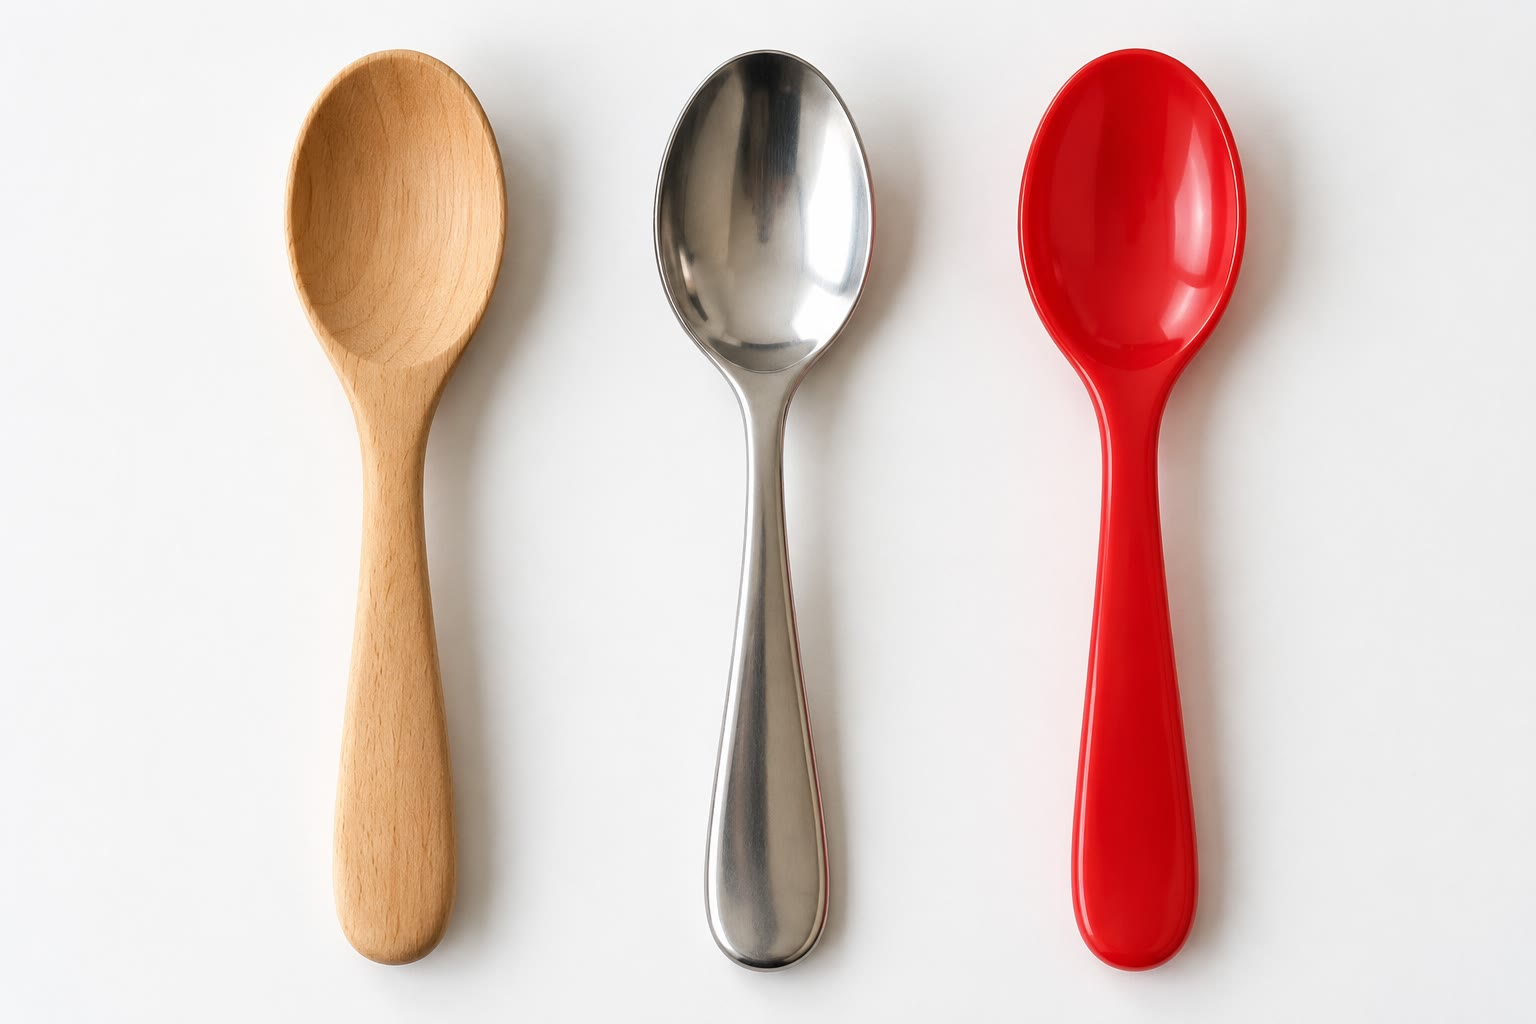
\includegraphics[width=0.55\linewidth]{images/book1/ai/g1-three-spoons.jpg}

{\small Tres cucharas: el mismo \omterm{def:g1:materials-around-us:object}{objeto}, tres \omterm{def:g1:materials-around-us:material}{materiales} --- madera, metal
y plástico.}
\end{omfigure}

\begin{example}[Un material, muchos objetos]\label{ex:g1:materials-around-us:wood}
La madera es el \omterm{def:g1:materials-around-us:material}{material} de un lápiz, de una silla, de una puerta, de
un tren de juguete y de una cuchara de palo. Muchos \omterm{def:g1:materials-around-us:object}{objetos} distintos
pueden estar hechos del mismo \omterm{def:g1:materials-around-us:material}{material}.
\end{example}

\begin{remark}[Objetos hechos de varios materiales]\label{rem:g1:materials-around-us:several}
Muchos \omterm{def:g1:materials-around-us:object}{objetos} están hechos de más de un \omterm{def:g1:materials-around-us:material}{material}. Unas tijeras tienen
las hojas de metal y los mangos de plástico. Un lápiz es de madera por
fuera y tiene dentro una barrita gris de grafito. Una ventana es de
vidrio, con un marco de madera, de metal o de plástico.
\end{remark}

\section{Siete materiales corrientes}

\begin{proposition}[Materiales por todas partes]\label{prop:g1:materials-around-us:seven}
Casi todos los \omterm{def:g1:materials-around-us:object}{objetos} que nos rodean están hechos de unos pocos
\omterm{def:g1:materials-around-us:material}{materiales} corrientes:
\begin{itemize}
  \item \textbf{madera}: mesas, sillas, lápices, puertas;
  \item \textbf{metal}: tenedores, llaves, clavos, sartenes, bicicletas;
  \item \textbf{vidrio}: ventanas, tarros, botellas, vasos;
  \item \textbf{plástico}: cuencos, botellas, juguetes, cubos;
  \item \textbf{papel} y cartón: libros, servilletas, cajas;
  \item \textbf{tela}: ropa, cortinas, bolsas --- hechas de lana,
        de algodón o de otros hilos;
  \item \textbf{piedra}: muros, escalones, guijarros, estatuas.
\end{itemize}
\end{proposition}

\begin{omfigure}
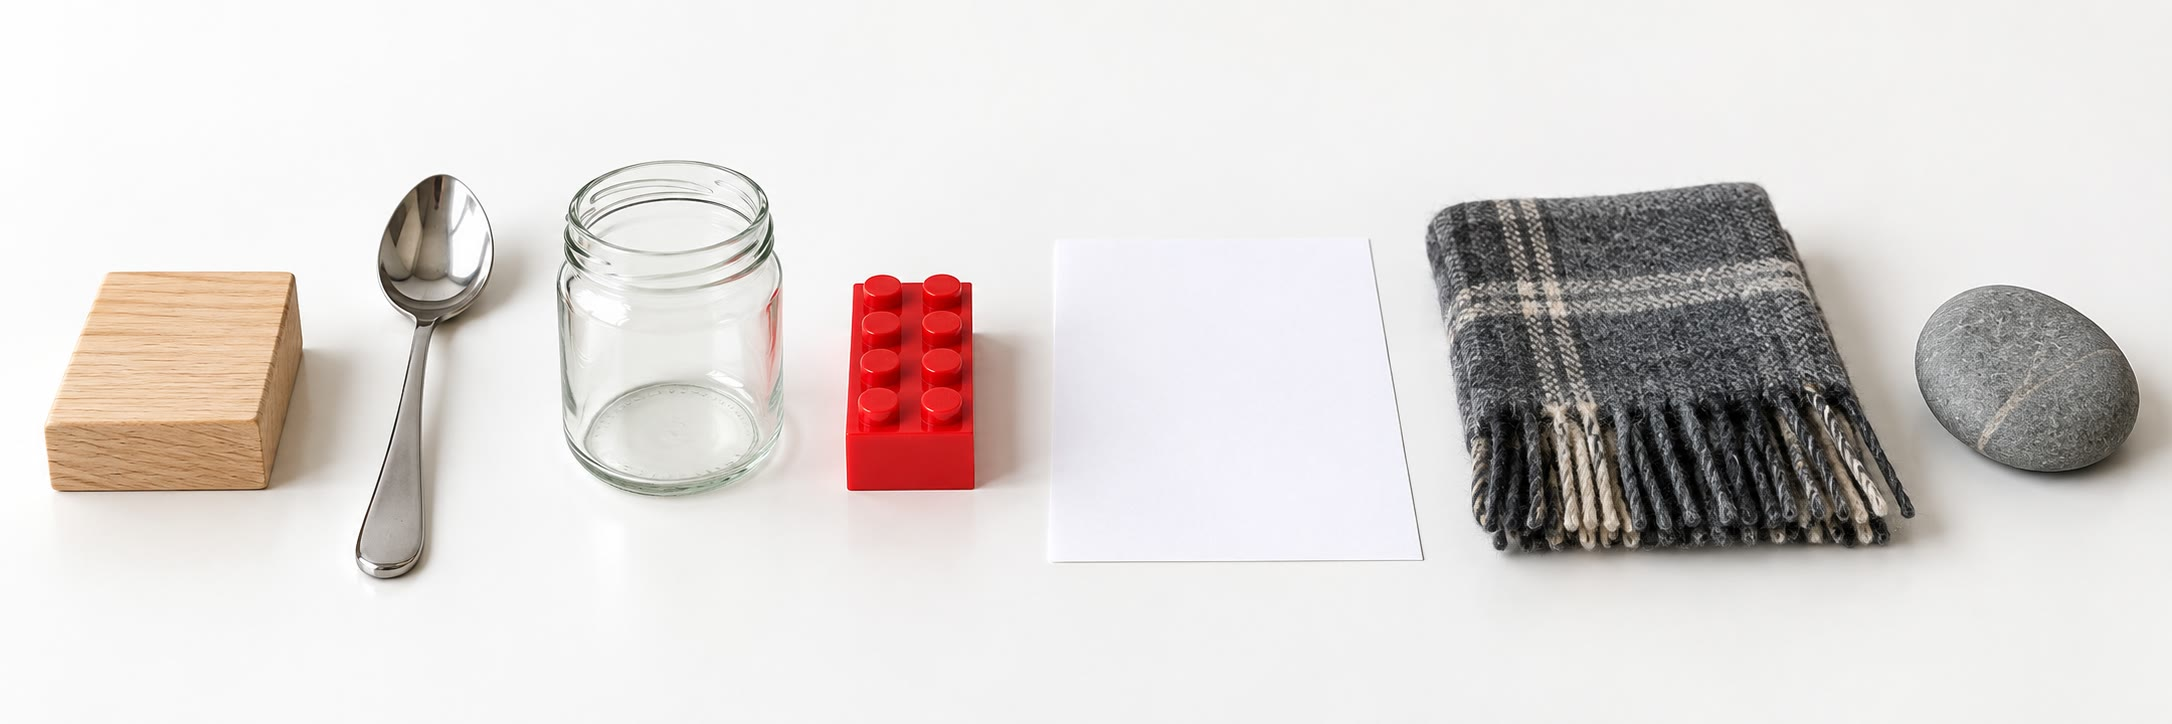
\includegraphics[width=0.75\linewidth]{images/book1/ai/g1-material-samples.jpg}

{\small Siete muestras, de izquierda a derecha: madera, metal, vidrio,
plástico, papel, tela (lana) y piedra.}
\end{omfigure}

\begin{remark}[Nombres que también son materiales]\label{rem:g1:materials-around-us:names}
A una hoja de papel la llamamos ``un papel'' porque está hecha de
papel, y al vidrio de una ventana lo llamamos a menudo ``el cristal''.
La palabra del \omterm{def:g1:materials-around-us:object}{objeto} y la palabra del \omterm{def:g1:materials-around-us:material}{material} son entonces la misma.
Cuando hablamos de \omterm{def:g1:materials-around-us:material}{materiales}, hablamos de aquello de lo que están
hechas las cosas, no del \omterm{def:g1:materials-around-us:object}{objeto}.
\end{remark}

\section{Propiedades de los materiales}

\begin{definition}[Propiedad de un material]\label{def:g1:materials-around-us:property}
Una \emph{propiedad de un material}\index{propiedad de un material} es
algo que podemos averiguar sobre él mirándolo, tocándolo o
poniéndolo a prueba: ¿es duro o blando? ¿Se ve a través de él? ¿Lo
atrae un imán? ¿Flota en el agua o se hunde?
\end{definition}

\begin{example}[Duro y blando]\label{ex:g1:materials-around-us:hard}
Un guijarro es duro: si lo apretamos con el pulgar, no queda ninguna
marca. Una bufanda de lana es blanda: se dobla y se pliega en la mano.
La madera, el metal, el vidrio y la piedra son duros; la tela y el
papel son blandos y se doblan con facilidad.
\end{example}

\begin{example}[Ver a través]\label{ex:g1:materials-around-us:see-through}
Vemos el jardín a través de una ventana: el vidrio deja pasar la luz, y
decimos que es \emph{transparente}. No podemos ver a través de una
puerta de madera, de una pared de ladrillo ni de una sartén de metal.
Algunos plásticos son transparentes, como una botella de agua; otros
no, como una pieza roja de un juego de construcción.
\end{example}

\begin{example}[Atraído por un imán]\label{ex:g1:materials-around-us:magnet}
Un imán atrae hacia sí un clip de acero, un clavo de acero o una llave
de hierro. No atrae la madera, el vidrio, el plástico, el papel, la
tela ni la piedra. Y, aunque sorprenda, no atrae todos los metales: una
lata de refresco de aluminio y un hilo de cobre se quedan donde están.
Un imán atrae los \omterm{def:g1:materials-around-us:object}{objetos} de hierro y de acero, que es casi todo hierro.
\end{example}

\begin{omfigure}
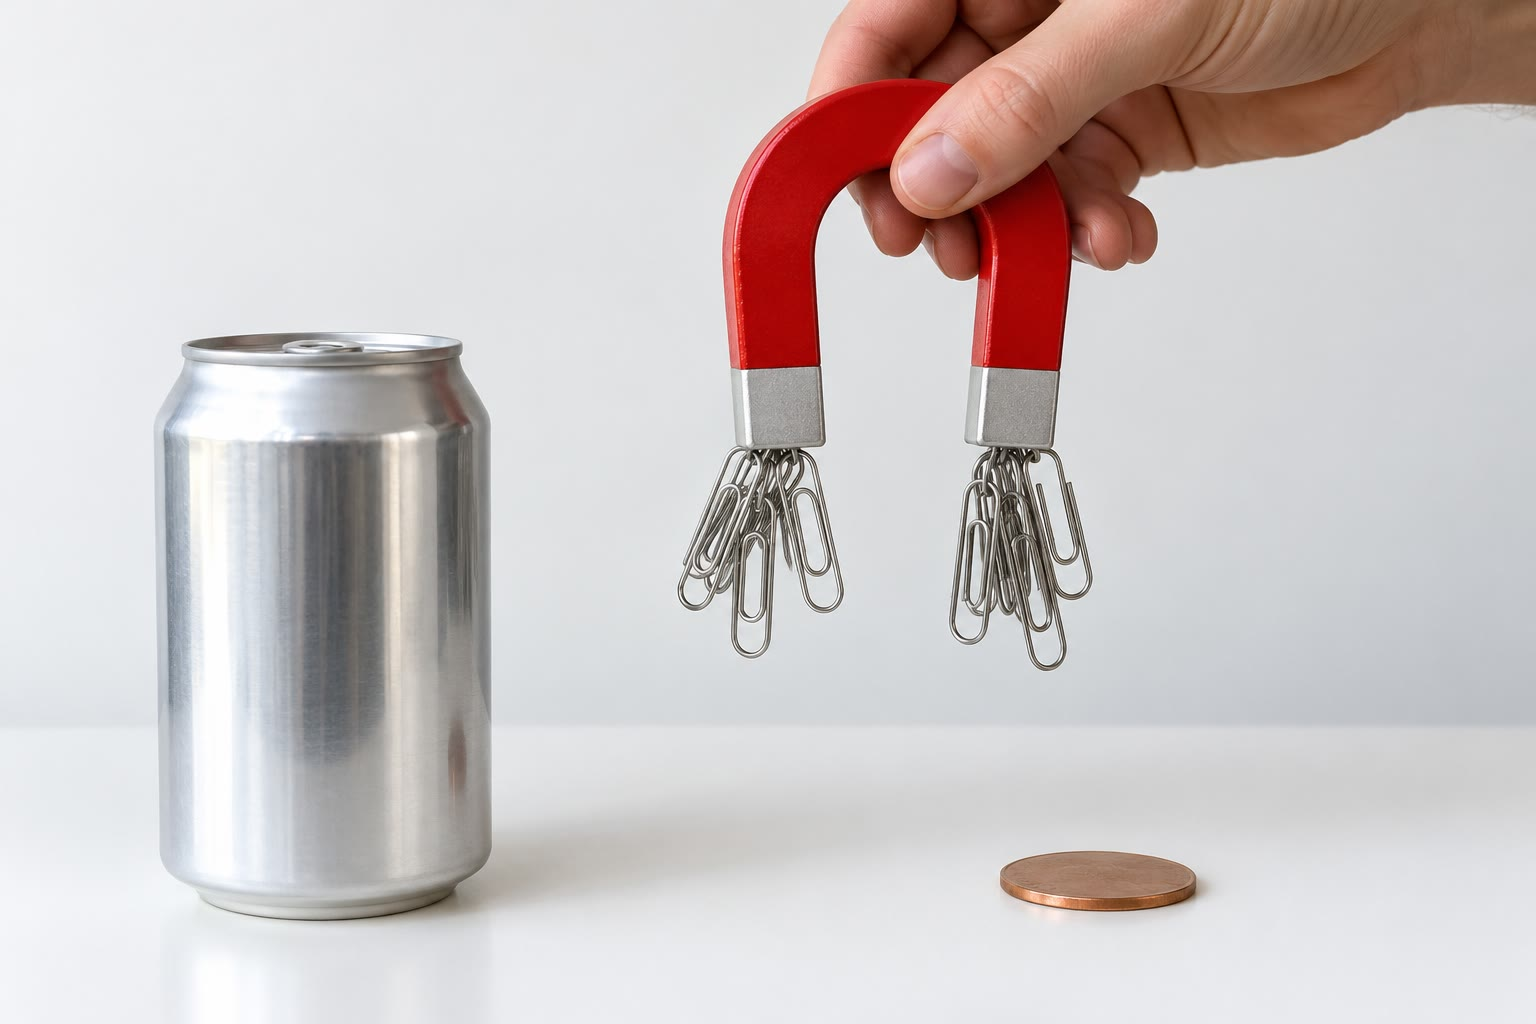
\includegraphics[width=0.55\linewidth]{images/book1/ai/g1-magnet-clips.jpg}

{\small Un imán levanta unos clips de acero. La lata de aluminio y el
disco de cobre que están sobre la mesa se quedan donde están.}
\end{omfigure}

\begin{example}[Flotar y hundirse]\label{ex:g1:materials-around-us:float}
Ponemos unos cuantos \omterm{def:g1:materials-around-us:object}{objetos} en un barreño con agua. Un taco de madera
y un tapón de plástico flotan. Un guijarro, una canica de vidrio y un
clavo de acero se hunden hasta el fondo. Que una cosa flote o se hunda
también es una propiedad de su \omterm{def:g1:materials-around-us:material}{material}.
\end{example}

\begin{omfigure}
\begin{tikzpicture}[font=\small]
  % the basin
  \fill[omWater!80] (0,0) rectangle (9,2.2);
  \draw[omGlass, line width=0.8pt] (-0.1,2.7) -- (0,2.6) -- (0,0) -- (9,0)
    -- (9,2.6) -- (9.1,2.7);
  % floating: wooden block, plastic cap
  \fill[brown!55, draw=brown!70!black] (0.8,2.0) rectangle (2.2,2.5);
  \fill[red!70, draw=red!50!black] (3.7,2.05) rectangle (4.3,2.35);
  % sunk: pebble, marble, nail
  \fill[black!35, draw=black!60] (5.0,0.25) ellipse (0.45 and 0.22);
  \shade[ball color=cyan!40] (6.5,0.2) circle (0.18);
  \fill[black!55] (7.6,0.06) rectangle (8.6,0.14);
  \fill[black!55] (7.52,0.02) rectangle (7.62,0.18);
  % labels
  \node[anchor=south] at (1.5,2.75) {taco de madera};
  \node[anchor=south] at (4.0,2.75) {tapón de plástico};
  \node[anchor=north] at (5.0,-0.1) {guijarro};
  \node[anchor=north] at (6.5,-0.1) {canica};
  \node[anchor=north] at (8.1,-0.1) {clavo};
  \node[anchor=west, align=left] at (9.3,2.2) {estos flotan};
  \node[anchor=west, align=left] at (9.3,0.2) {estos se hunden};
\end{tikzpicture}

{\small En un barreño con agua: el taco de madera y el tapón de plástico
flotan; el guijarro, la canica de vidrio y el clavo de acero se hunden.}
\end{omfigure}

\section{Clasificar materiales}

\begin{method}[Clasificar según una propiedad]\label{met:g1:materials-around-us:sort}
Para clasificar un montón de \omterm{def:g1:materials-around-us:object}{objetos}:
\begin{enumerate}
  \item elige \textbf{una sola} pregunta, por ejemplo ``¿Lo atrae un
        imán?'';
  \item pon a prueba cada \omterm{def:g1:materials-around-us:object}{objeto} y colócalo en el grupo del ``sí'' o en
        el grupo del ``no'';
  \item después, si quieres, vuelve a clasificar cada grupo con otra
        pregunta.
\end{enumerate}
Una pregunta cada vez: así cada \omterm{def:g1:materials-around-us:object}{objeto} tiene exactamente un sitio.
\end{method}

\begin{omfigure}
\begin{tikzpicture}[font=\small]
  \draw[omDef, line width=1pt] (0,0) circle (2.3);
  \draw[omProp, line width=1pt] (2.4,0) circle (2.3);
  \node[omDef, font=\small\bfseries] at (-0.6,2.65) {de metal};
  \node[omProp, font=\small\bfseries] at (3.0,2.65) {lo atrae un imán};
  \node[font=\footnotesize] at (-1.1,0.35) {lata};
  \node[font=\footnotesize] at (-1.1,-0.35) {hilo de cobre};
  \node[font=\footnotesize] at (1.2,0.6) {clavo de acero};
  \node[font=\footnotesize] at (1.2,0) {llave de hierro};
  \node[font=\footnotesize] at (1.2,-0.6) {clip};
  \node[font=\footnotesize] at (3.5,0) {(nada)};
  \node[anchor=west] at (5.2,0.9) {cuchara de palo};
  \node[anchor=west] at (5.2,0.3) {canica de vidrio};
  \node[anchor=west] at (5.2,-0.3) {bufanda de lana};
  \node[anchor=west] at (5.2,-0.9) {guijarro};
\end{tikzpicture}

{\small Dos preguntas, dos aros. Dentro del aro azul: los \omterm{def:g1:materials-around-us:object}{objetos} de
metal. Dentro del aro naranja: los \omterm{def:g1:materials-around-us:object}{objetos} que atrae un imán. En los
dos aros: los \omterm{def:g1:materials-around-us:object}{objetos} de hierro o de acero. Fuera de los dos: todo lo
demás.}
\end{omfigure}

\begin{center}
\small
\begin{tabular}{lccc}
\hline
\omterm{def:g1:materials-around-us:object}{objeto} (\omterm{def:g1:materials-around-us:material}{material}) & ¿duro? & ¿transparente? & ¿lo atrae un imán? \\
\hline
taco (madera) & sí & no & no \\
clavo (acero) & sí & no & sí \\
canica (vidrio) & sí & sí & no \\
tapón (plástico) & sí & no & no \\
hoja (papel) & no & no & no \\
bufanda (lana) & no & no & no \\
guijarro (piedra) & sí & no & no \\
\hline
\end{tabular}
\end{center}

\section{El material adecuado para cada uso}

\begin{proposition}[Cada material se elige por sus propiedades]\label{prop:g1:materials-around-us:choose}
Las personas eligen el \omterm{def:g1:materials-around-us:material}{material} de un \omterm{def:g1:materials-around-us:object}{objeto} según lo que el \omterm{def:g1:materials-around-us:object}{objeto}
tiene que hacer:
\begin{itemize}
  \item una ventana tiene que dejar entrar la luz: es de vidrio, que es
        transparente;
  \item un impermeable tiene que impedir que entre la lluvia y poder
        doblarse: es de plástico o de una tela que el agua no atraviesa;
  \item una sartén no debe fundirse en el fuego: es de metal;
  \item el mango de una sartén no debe quemar la mano: suele ser de
        madera o de un plástico duro, que no se calientan tanto como el
        metal;
  \item una almohada tiene que ser blanda: es de tela y está rellena de
        plumas o de fibras.
\end{itemize}
\end{proposition}

\begin{example}[Un barco]\label{ex:g1:materials-around-us:boat}
Un barco de juguete tiene que flotar. Puede ser de madera o de
plástico. Un barco hecho de un bloque macizo de piedra se hundiría
enseguida.
\end{example}

\begin{remark}[Vidrio roto]\label{rem:g1:materials-around-us:glass}
El vidrio es duro, pero se rompe, y sus trozos cortan. Cuando se rompe
un vaso, es un adulto quien recoge los trozos.
\end{remark}

\section{Ejercicios}

\begin{exercise}[$\star$]\label{exo:g1:materials-around-us:1}
¿Una silla es un \omterm{def:g1:materials-around-us:object}{objeto} o un \omterm{def:g1:materials-around-us:material}{material}? ¿Y la madera, es un \omterm{def:g1:materials-around-us:object}{objeto} o un
\omterm{def:g1:materials-around-us:material}{material}?
\end{exercise}

\begin{exercise}[$\star$]\label{exo:g1:materials-around-us:2}
Nombra el \omterm{def:g1:materials-around-us:material}{material} de cada \omterm{def:g1:materials-around-us:object}{objeto}: el cristal de una ventana, un clavo,
un guijarro, un libro, un calcetín.
\end{exercise}

\begin{exercise}[$\star$]\label{exo:g1:materials-around-us:3}
Da dos \omterm{def:g1:materials-around-us:object}{objetos} hechos de madera y dos \omterm{def:g1:materials-around-us:object}{objetos} hechos de plástico.
\end{exercise}

\begin{exercise}[$\star$]\label{exo:g1:materials-around-us:4}
Busca el intruso y explica por qué: una cuchara de palo, un tenedor de
metal, una cuchara de plástico, una silla de madera. (Fíjate en los
\omterm{def:g1:materials-around-us:material}{materiales}.)
\end{exercise}

\begin{exercise}[$\star$]\label{exo:g1:materials-around-us:5}
¿A través de qué \omterm{def:g1:materials-around-us:material}{material} podemos ver: la madera, el vidrio o la
piedra?
\end{exercise}

\begin{exercise}[$\star$]\label{exo:g1:materials-around-us:6}
Acercamos un imán a un clavo de acero, a una canica de vidrio y a un
taco de madera. ¿Cuál de ellos atrae?
\end{exercise}

\begin{exercise}[$\star$]\label{exo:g1:materials-around-us:7}
Mira la figura del barreño. ¿Cuántos \omterm{def:g1:materials-around-us:object}{objetos} flotan? ¿Cuántos se
hunden?
\end{exercise}

\begin{exercise}[$\star$]\label{exo:g1:materials-around-us:8}
Unas tijeras tienen hojas y mangos. ¿De qué \omterm{def:g1:materials-around-us:material}{material} está hecha cada
parte? ¿Las tijeras están hechas de un \omterm{def:g1:materials-around-us:material}{material} o de dos?
\end{exercise}

\begin{exercise}[$\star$]\label{exo:g1:materials-around-us:9}
Mira la figura de los dos aros. ¿En qué aro está la lata de refresco?
¿Por qué no está en el aro naranja?
\end{exercise}

\begin{exercise}[$\star\star$]\label{exo:g1:materials-around-us:10}
¿Por qué las ventanas son de vidrio y no de madera?
\end{exercise}

\begin{exercise}[$\star\star$]\label{exo:g1:materials-around-us:11}
Sam quiere clasificar estos 8 \omterm{def:g1:materials-around-us:object}{objetos} con la pregunta ``¿Lo atrae un
imán?'': un clavo de acero, un clip, un guijarro, una cuchara de palo,
una llave de hierro, una lata de refresco, una canica de vidrio y un
calcetín de lana. ¿Cuántos \omterm{def:g1:materials-around-us:object}{objetos} van al grupo del ``sí''? ¿Cuántos al
grupo del ``no''?
\end{exercise}
